\documentclass[10pt,a4paper]{article}
\usepackage[utf8]{inputenc}
\usepackage{amsmath}
\usepackage{amsfonts}
\usepackage{amssymb}
\usepackage{graphicx}
\usepackage{color}
\usepackage{float}
\usepackage{gensymb}

\usepackage{eurosym}
 
\usepackage{fancyhdr}
 
\pagestyle{fancy}
\fancyhf{}
\rhead{Amsterdam university of applied sciences}
\lhead{Swarming: Research}
\rfoot{Page \thepage}


%\usepackage{draftwatermark}
%\SetWatermarkText{Concept}
%\SetWatermarkScale{5}

\definecolor{codegreen}{rgb}{0,0.6,0}
\definecolor{codegray}{rgb}{0.5,0.5,0.5}
\definecolor{codepurple}{rgb}{0.58,0,0.82}
\definecolor{backcolour}{rgb}{0.95,0.95,0.92}
\usepackage{listings}
\lstdefinestyle{cstyle}{
    backgroundcolor=\color{backcolour},   
    commentstyle=\color{codegreen},
    keywordstyle=\color{magenta},
    numberstyle=\tiny\color{codegray},
    stringstyle=\color{codepurple},
    basicstyle=\footnotesize,
    breakatwhitespace=false,         
    breaklines=true,                 
    captionpos=b,                    
    keepspaces=true,                 
    numbers=left,                    
    numbersep=5pt,                  
    showspaces=false,                
    showstringspaces=false,
    showtabs=false,                  
    tabsize=2
}
\graphicspath{ {./images/} }

\begin{document}
\begin{titlepage}
    \centering
    \vfill
    {\Large

    Swarming\\

   
    {\small Research document}\\
    {\small Version 1.0}\\
    {\small \today}\\
        
        \vskip2cm
        {\small M. van Wilgenburg, W. Mukhtar, E. van Splunter, M. Siekerman, T. Zaal and M. Visser}\\
    }    
    \vfill
%    \includegraphics[width=1\textwidth]{WireS4}
    
    \vfill
    \vfill
\end{titlepage}

\newpage

\listoffigures
\newpage

\listoftables
\newpage

\tableofcontents
\newpage

\section{What do we consider swarming?}
Swarming is a wide concept and can be achieved in many forms. In this section will be defined what we consider swarming during this project. Many choices made here will be up for discussion, but these choices have to be made so the project can be successfully specified. For example, no clear minimal number of units is specified for a group of robots to be called a swarm. When specification have to be exact and testable this becomes a problem. The following subjects will be discussed: number of robots and scalability, precision of localisation. Its important to keep in mind that the choices made in this section, mostly consist of educated guesses. These guesses will later be confirmed by testing.

\subsection{Situational sketch}
To be able to make any assumptions we will first sketch a situation. We propose a test situation where a swarm of eight robots need to explore a room as efficient as possible. They will need to find a certain object and when the object is found by one of the units, the others will have to come to the objects location. For the robots to search efficiently they will need some type of "close range" relative localisation, so they can spread evenly across the room without bumping into each other. Speed is also an important factor when considering the frequency of distance measurements. For this sketch we chose an average speed of 3,6km/h or 1m/s, this a bit slower than average walking speed and seems realistic for smaller robots. The robots are programmed to keep a distance of 5cm from each others outer boundaries. And should keep a absolute minimal distance of 2cm.

\subsection{Precision of localization}
An obvious answer for the question "How precise does the localisation need to be?" would be "As precise as possible!". However with swarming robots it might not need to be precise at all. This depends mostly on what the swarm needs to accomplish. For the situation we proposed the localisation needs to be precise at closer range but can be less accurate when further away. We choose to define "close range" as 0 to 3 meters, and "long range" as 3 to 25 meters (further if possible).  The big difference between the two is the margin of error that is allowed. \\

Close range localisation has a smaller margin of error because the robots will need to be able to move precisely, to perform certain tasks without bumping into each other. To determine the precision needed, size of the robots matter.  The project group of the Zebro light set out to make a robot with maximum dimensions of  300x 200 x 60 mm \cite{zebrolight}. When the swarming module is placed in the middle of this platform the the absolute minimum distance between the two modules will be 20cm from middle point till middle point. Considering that some deviations might occur the minimal measuring distance or "dead zone" is chosen to be 15cm. The worst case scenario is shown in figure \ref{fig:smrange} the maximum deviation is calculated with by dividing the absolute minimal distance (2cm) by the distance between the swarming modules (22cm). This results in a maximum deviation of 9\% in the close range distance measurement. The relative angle to another swarming module is needed to successfully implement localisation. At close range the localisation will mostly by used so the robots don't collide, or to implement swarming behaviour like trail following as discussed in the problem definition. Limited information about the relative angle would be enough to perform these tasks. We propose angle measurement at close range to have a resolution of 45\degree. In field testing will have to validate these assumptions. The speed of the robots determine the frequency at which the close range localisation should take place. The robots in this sketch move at a maximum speed of 1 m/s, the worst case scenario is that the robots will approach each other head-on. This makes their combined speed 2 m/s. The robots have been programmed to keep a minimal distance of 5cm from each other. Dividing the minimal distance by the combined speed will result in 40Hz which is the minimal required sampling speed. \\

\begin{figure}[H]
        \centering
        \graphicspath{ {./images/} }
        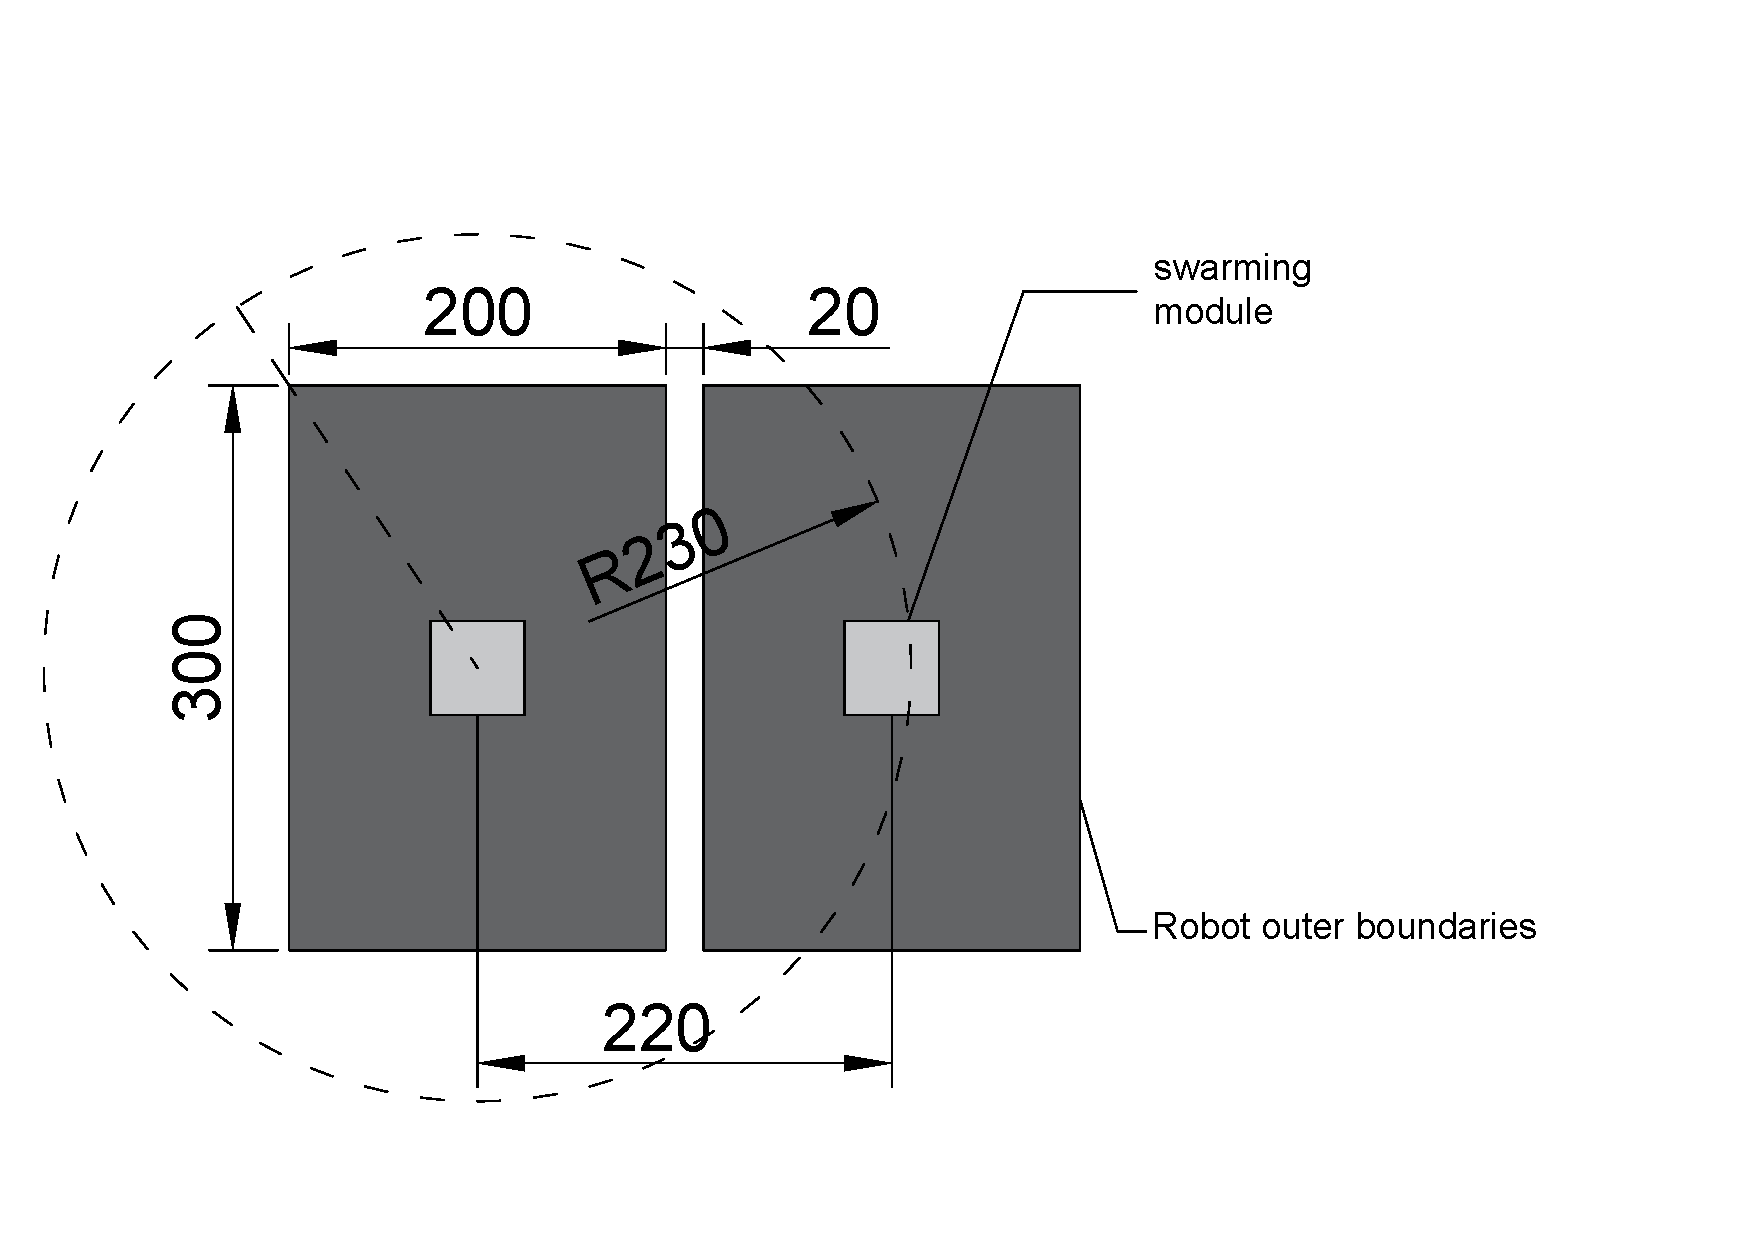
\includegraphics[scale=.3]{smrange.pdf}
        \caption{Worst case scenario for two Zebro light robots at close range}
        \label{fig:smrange}
\end{figure}


Long range localisation will only be used to keep members of certain groups in the swarm together. When the units are working together on a task, they will be using the close range localisation. A situation might occur where a members of a group of members of the swarm will have to complete a task outside of the range of the close range localisation. When they are done and they want to return to the swarm the long range localisation will be used. As discussed earlier the long range localisation will start at three meters. But it has to get the unit in close range. Therefore the minimal measuring distance will be chosen at two meters. The distance measurement will need to be precise enough to detect when it reaches the overlap between 2 and 3 meters. This maximum deviation for this to be true is 1 meter. Long range localisation will actually be a long range distance measurement. The relative angle between modules will not be needed. When an unit needs to return to the rest of the swarm a algorithm can be developed that finds it way back by looking at the changing distance. When the robot is trying to determine the right direction, the update frequency is important. At far range we would assume that a robot has to move one meter to determine if its getting closer or not. With the robot moving at 1 m/s the minimal update frequency is 1Hz. \\\\
Summed up the specifications of localisation are:


% Please add the following required packages to your document preamble:
% \usepackage{graphicx}
\begin{table}[h]
\centering
\resizebox{\textwidth}{!}{%
\begin{tabular}{|l|l|l|}
\hline
                     & \textbf{Close range (0 - 3 m)} & \textbf{Long range (3 - 25m)} \\ \hline
Deadzone distance    & 0,015 meters                   & 2 meters                      \\ \hline
Deviation (distance) & +/- 9\%                         & +/- 1 meter                   \\ \hline
Angle Resolution     & 45\%                            & -                             \\ \hline
Update frequency     & 40Hz                           & 1Hz                           \\ \hline
\end{tabular}%
}
\caption{Localisation specification}
\label{smrange}
\end{table}



\subsection{Number of units of the Swarm}
As discussed before in the problem definition, its hard to put an exact number on what number of units it required to form a swarm. We mentioned "a high number of units" and that a minimum number of units is hard to justify. We will look at what the preferable amount of units would be to demonstrate the swarming module. Also we will look at a minimum amount and a maximum. Important to remember is that the swarm must always be scalable, so no static number of units will be defined.\\\\Robots in a swarm have limited capabilities on their own, thus they need to work together to perform a complicated task. When one unit breaks down the others should still be able to complete the task. With this is mind the absolute minimum units required for a swarm is chosen to be 3. When one breaks down the other two can still complete the task faster/better than one could do on its own. It would be preferable to make the total swarm endlessly scalable. When developing the swarming module no maximum number should be defined to the swarm. Hardware limitations will later determine a maximum. However a maximum of units can be calculated, that one unit has to be able to detect at close range. The detection surface can be viewed as a circle around of unit with a radius of 3 meters. The radius for the  circle is also calculated for the area where robots will avoid each other. This is done by taking the furthest point seen from the center of the robot and then adding 0,05m (the range where robots will avoid each other), this circle is shown in figure \ref{fig:smrange}. The maximum amount of robots in this range can then be calculated using a simple tool, the result is shown in figure \ref{fig:ccircle}. The end result is a maximum of 130 robots.

\begin{figure}[H]
        \centering
        \graphicspath{ {./images/} }
        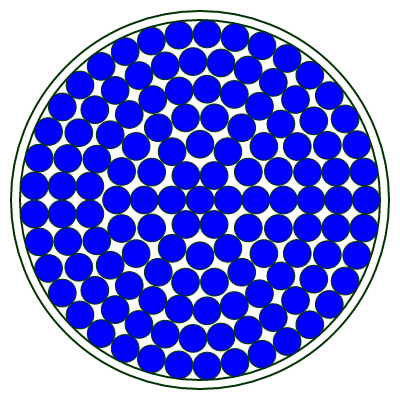
\includegraphics[scale=.6]{ccircle.png}
        \caption{Maximum amount of robots within the close range radius, the maximum amount results in 130.}
        \label{fig:ccircle}
\end{figure}



 For the sake of demonstration we would like to recreate the "feel" of a swarm. This means a higher number of units is required. We chose this number to be between 6 and 12 units depending on the time and budget. 

\begin{table}[h]
\centering
\resizebox{\textwidth}{!}{%
\begin{tabular}{|l|l|l|l|l|}
\hline
 & \textbf{minimum} & \textbf{maximum} & \textbf{maximum (close range)} & \textbf{Preferred (demonstration)} \\ \hline
Number of Units & \multicolumn{1}{c|}{3} & \multicolumn{1}{c|}{$\infty$} & \multicolumn{1}{c|}{130} & \multicolumn{1}{c|}{6 to 12} \\ \hline
\end{tabular}%
}
\caption{Specifications number of units}
\label{specunits}
\end{table}


\section{Protocol}
\subsection{Hardware}

For the internal communication between the different systems there are multiple protocols to chose from to transmit data. every subsystem with a microcontroller should be able to communicate with the rest of the system. Because every system should be able to share their information it is necessary to have a multimaster system which allows every system to share their information without being dependent on a single master. To see which protocols are viable multiple protocols will be compared.

Building a modular robot consisting of subsystems, there must be a method to let these "\textit{subsystems}" communicate with each other to exchange relevant information. 

Every subsystem features a micro-controller which must be capable of transmitting and receiving data.  

\subsubsection{TWI}
The name TWI stands for "Two wire interface" which strongly resembles Phillps' protocol $I^(2)C$. Like the name suggests the bus is build up using two wires, one is used for the clock signal and the other is used for the data signal. Each of these wires is connected to the powerline through a pull-up resistor so every subsystem connected to the line can pull the line down which other systems can see. TWI can be used as a multimaster system which means every subsystem can send it's data without being dependend on a single master.



\begin{figure}[H]
        \centering
        \graphicspath{ {./images/} }
        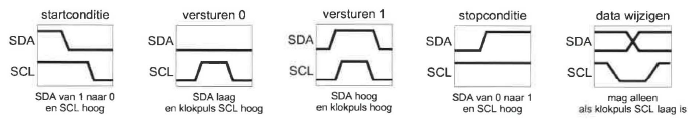
\includegraphics[scale=.6]{datacondities}
        \caption{Data conditions}
        \label{fig:Data conditions}
\end{figure}
In the above figure multiple data and clock combinations are shown, these combinations define the message start, sending a zero, a one and a stopbit. The system that wants to send information starts a message bij changing the datasignal from one to zero on a high clocksignal. All systems that are listening now know one of the systems is going to send a message. Data can be send by changing the dataline from zero to one or the other way around during a low clocksignal, the other systems will read this bit when the clocksignal becomes high again. Once the system is done sending its message it will let the other systems know by sending a stopbit.

\begin{figure}[H]
        \centering
        \graphicspath{ {./images/} }
        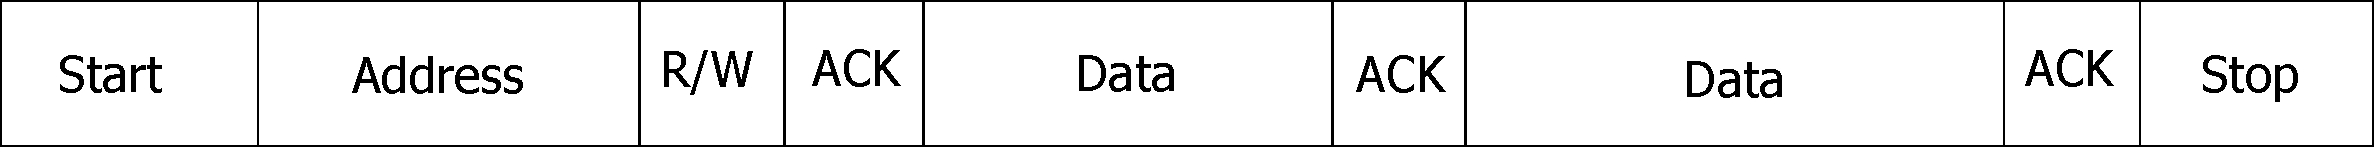
\includegraphics[scale=.6]{TWImessage}
        \caption{Structure of a TWI message}
        \label{fig:TWIstructure}
\end{figure}
In the above picture the structure of a message is shown. As explained before the message starts with a startbit after which a small header follows. The header contains information about who is going to be adressed by the message and if you want to read or write. After this the adressed system will respond with an acknowladge to make sure the information has come across. When the acknowladge is recieved the system will start sending data, followed by and acknowladge from the reciever after every recieved byte of data. when the system is done sending all of its data and recieved the last acknowladge it will send the stopbit which means all communication has ended.
\\
\\
TWI has a few benefits, because it is a simple serial protocol it only uses two wires. this saves a lot of space in the hardware design. Also, it has the possibility to be used as a multimaster system.
The speed of the communication depend on the frequency of the controller that will be used.


\subsubsection{SPI}
SPI or Serial Peripheral Interface is, like it names suggests, a serial interface. This interface can be connected in two ways, each having its own advantage. How this works will be explained using the following figure.
% \begin{figure}[H]
%         \centering
%         \graphicspath{ {./images/} }
%         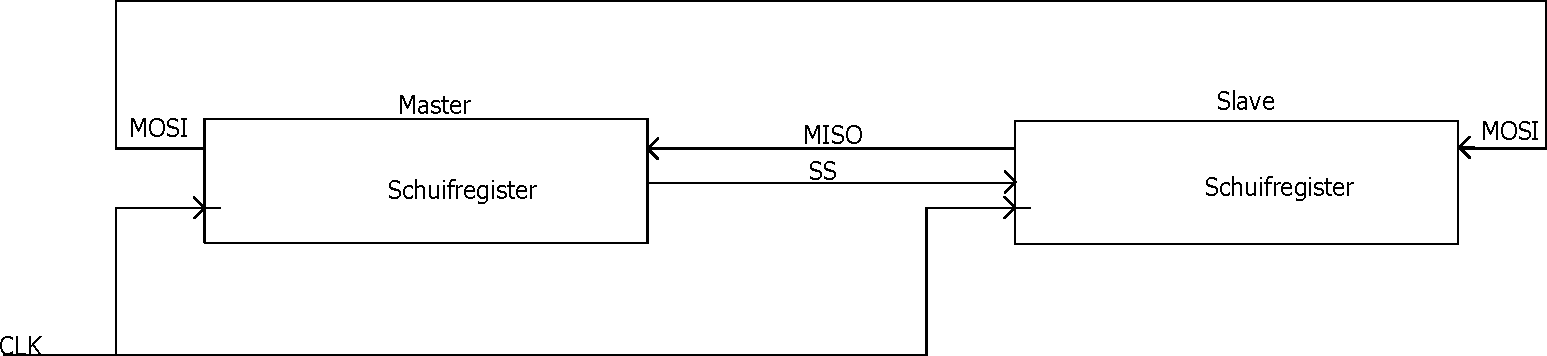
\includegraphics[scale=.6]{SPI}
%         \caption{SPI connections}
%         \label{fig:SPIconnections}
% \end{figure}

\subsubsection{UART}
\subsection{Software}


\newpage
\section{Localization}
Building a swarm of robots, location awareness may be required to ensure an more efficient operation. Implementing location awareness into a swarm of robots could result in better cooperation. For example: exploration based tasks can be executed on a much lower time scale. With location awareness the swarm can spread out evenly making sure that every part of the perimeter will be explored thoroughly. 

With location awareness it is also possible to divide the swarm into multiple groups. Because the location of every individual is available these individual groups can be formed very quickly by selecting the nearest unit. This also enables quick assists when an individual robot gets stuck or needs to execute a task that require more than one unit.

For mapping the various positions of all robots in a swarm a localization technique needs to be implemented. The robots can use information as relative position and relative orientation of their neighbours to interpret and fuse the information collected by other robots. With relative position the units can define the distance relative to each other. When all robots in the swarm are aware of the distance opposite to each other a map of the current formation can be created. However this can result in multiple solutions because there are no orientations involved. This means that the map could be mirrored. As seen in in Fig \ref{Angle}


\begin{figure}[H]
\centering
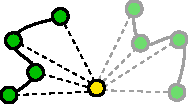
\includegraphics[width=0.5\textwidth]{drolletje.pdf}
\caption{Stationary robot (yellow) cannot compute the relative position of the moving robot (green), since all distance measurements (dashed lines) are invariant to rotations around the stationary robot.\cite{Angle}}
\label{Angle}
\end{figure}

For the robots to know in what direction the measured distance is applicable to, they can analyze the change in distance after a robot has moved a specific direction. In order to leverage the previous trilateration procedure requires coordinating the motion of the robots in a manner that gives every robot a chance to move and ensures that when a robot is moving its neighbours remain stationary. \cite{Angle}
This can be seen in figure \ref{Range} 

\begin{figure}[H]
\centering
\includegraphics[width=0.3\textwidth]{range.pdf}
\caption{Moving robot (yellow) can analize the direction of the moving robot (green), as a result of the movement (arrows) of the yellow robot, the relative distance has changed.}
\label{Range}
\end{figure}

This can also be achieved by the use of stationary beacons. When a minimum of three beacons is placed on the field location of the robots within this field can be measured, this is called triangulation. Triangulation is the process of determining the location of a point by measuring angles to it from known points. This is illustrated in figure \ref{triangulation}.

\begin{figure}[H]
\centering
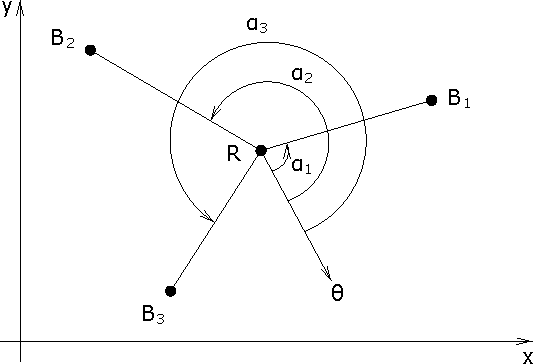
\includegraphics[width=0.7\textwidth]{triangulation.pdf}
\caption{Triangulation setup in a 2D field. R denotes the robot. B1, B2, and B3 are the beacons.$ \alpha_1$, $\alpha_2$, and $\alpha_3$ are the angle measurements respectively for B1, B2, and B3, relatively to the robot reference orientation $\phi$. \cite{triangulation}}
\label{triangulation}
\end{figure}

A more efficient solution is to retrieve the relative orientation opposite to each other. In combination with the relative distance every robot knows the exact relative position of all the other robots in range of the network.

\begin{figure}[H]
\centering
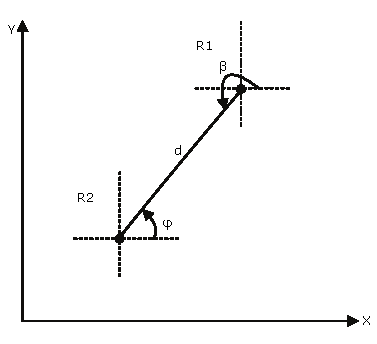
\includegraphics[width=0.6\textwidth]{orientation.pdf}
\caption{relative localization system using relative distance and orientation}
\label{orientation}
\end{figure}

As seen in figure \ref{orientation} each robot has a common reference direction, the direction relative to this reference is called the relative orientation of the robot and can be visualized as shown in figure \ref{orientation}. With the known distance ‘d’, the mapping of the swarm can be completed.
\newpage

\subsection{Relative Distance}
Relative distance can be measured using various methods. The most common methods are \textit{"Received Signal Strength Indication"} and \textit{"Time Of Flight"} abbreviated as RSSI and TOF. 

\subsubsection{Received Signal Strength}
A method to determine distance can be implemented using Received Signal Strength abbreviated as "RSSI". Typically RSSI is a measure of dBm, which is ten times the logarithm of the ratio of the power (P)
at the receiving end and the reference power (Pref). Power at the receiving end is inversely proportional to the
square of distance.\cite{RSSI} Hence RSSI could potentially be used as an indicator of the distance
at which the sending unit (robot) is located from the receiving unit.\cite{RSSI}

RSSI is defined as ten times the logarithm of the ratio of power of the received signal
and a reference power (for example 1mW). It is known that power dissipates from its source
as it moves further out. As mentioned earlier the relationship between power and distance is that power is inversely
proportional to the square of the distance travelled. \cite{RSSI}

In theory it seems as a suitable implementation for the purpose, determining relative distance between
different units. However various test results have shown that RSSI is only reliable under certain circumstances.
Test results have shown that if the orientation of the sending or receiving unit changes it becomes very unreliable.
The graphs below show the reliability of RSSI when the direction is being altered.\cite{RSSI}

\begin{figure}[H]
\centering
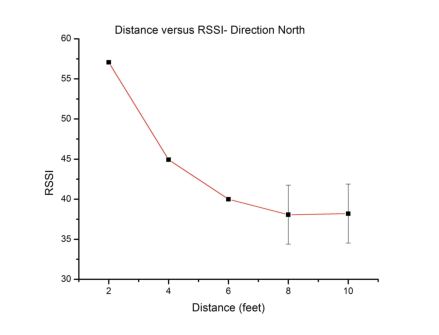
\includegraphics[width=0.9\textwidth]{North.pdf}
\caption{Distance versus RSSI plot showing inverse non linear
relationship.\cite{RSSI}}
\label{North}
\end{figure}

\begin{figure}[H]
\centering
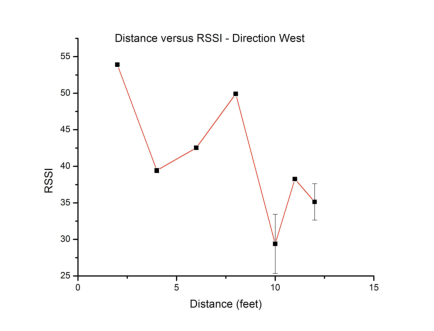
\includegraphics[width=0.9\textwidth]{West.pdf}
\caption{Distance versus RSSI plot showing lack of
reliability when tested in a different direction.\cite{RSSI}} 
\label{West}
\end{figure}

\begin{figure}[H]
\centering
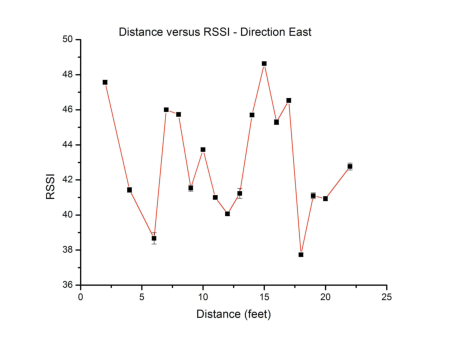
\includegraphics[width=0.9\textwidth]{East.pdf}
\caption{Distance versus RSSI plot showing lack of
reliability when tested in a different direction.\cite{RSSI}} 
\label{East}
\end{figure}
\newpage


Even though RSSI was very promising in many studies, through multi directional experiments it became clear that even under ideal conditions with weather and interference controlled, the RSSI data could not be relied upon. At times the data was correct showing the expected inverse square relation with distance and at other times it didn't.\cite{RSSI}


\subsubsection{Time Of Flight}
Another common method to determine relative distance is Time Of Flight abbreviated as "TOF". Time Of Flight describes a method that measures the time that an particular wave takes to travel a distance trough a medium. The wave can be acoustic, electromagnetic and light.

For relative distance measurements Time Of Flight is often combined with Time Difference Over Arrival abbreviated as "TDOA". Combining these methods enables relative distance measurements to specific units/nodes. TDOA measures the time difference between the transmission and arrival of a wave. With the velocity of propagation times the travelled time de relative distance between two or more nodes can be determined. However TOF also features certain limitations being clock synchronization, noise, sampling and multipath channel effects.\cite{TOF} 
\\\\
\textit{Clock Synchronization}
TOF ranging systems need to estimate the time of transmission and arrival and comparing this with a common time reference.\cite{TOF} If the different time references are not perfectly synchronized a time offset error occurs. With the faster the propagation speed, the greater the error in distance. 
\\\\
\textit{Sampling}
Using Light or electromagnetic waves to determine the relative distance can add several limitation. Due to the high velocity propagation (being nearly equal to equal of the velocity propagation of light) sampling this signal requires very high clock rates to do so. It would take a 15GHz clock to achieve one centimetre resolution.\cite{Arduino}

in the 1960's, Tektronix invented a sampling method with a oscilloscope that could measure signals in the GHz range without using high speed clocks. This method is called Sequential Equivalent Time Sampling abbreviated as "SETS". The SETS acquires one sample per trigger see figure \ref{SETS}. When a trigger is detected a sample is taken after a very short, but well defined delay. When the next trigger occurs a small time increment "Delta T" is added to this delay and the digitizer takes another sample. This process is repeated many times with "Delta T" added to each previous acquisition, until the time windows is filled.\cite{SETS} In figure \ref{SETS2} another example of an sinusoidal signal is displayed using the SETS method. 

Using the SETS method enables the use of waveform with an velocity propagation nearly equal to equal to the speed of light. However implementing a advanced SETS circuit is required to reach accuracy of less than 1 meter indoors.\cite{TOF} However using waveforms with a high velocity propagation enables faster data transfers and a larger range.\cite{TOF}

\begin{figure}[H]
\centering
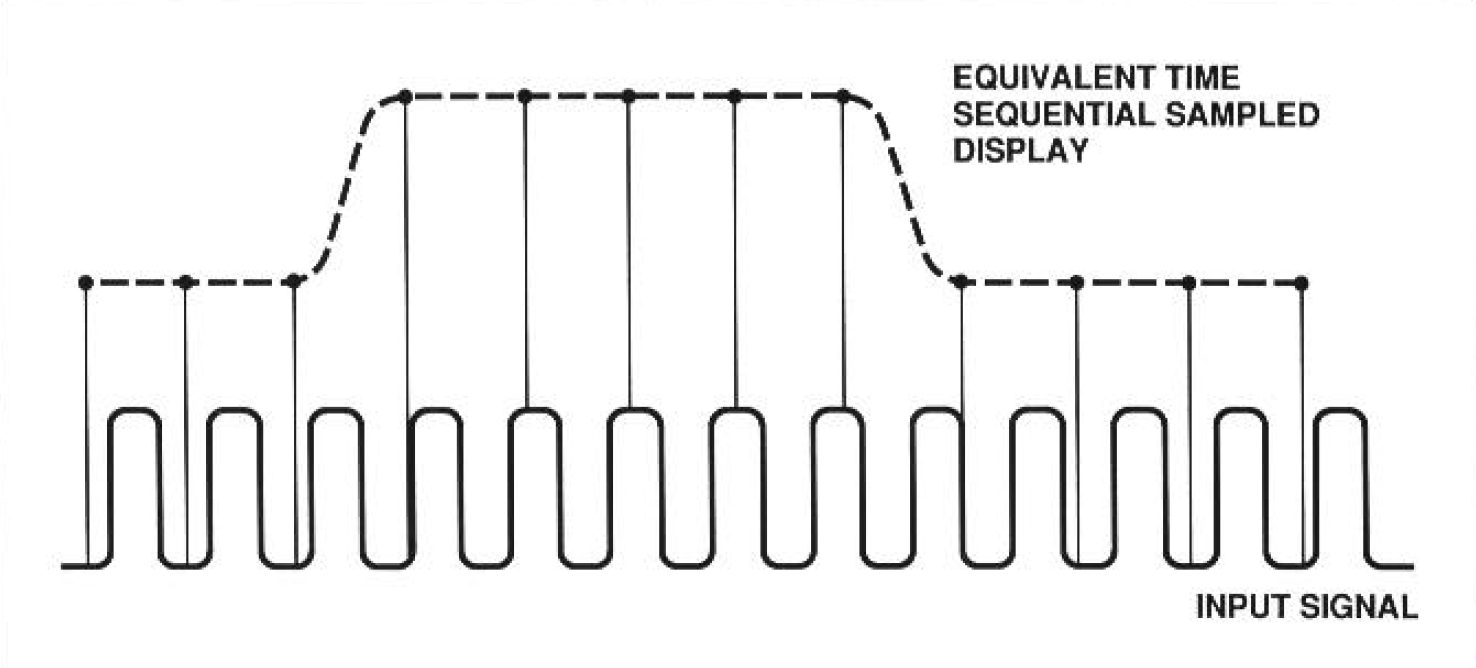
\includegraphics[width=0.9\textwidth]{SETS.png}
\caption{In sequential equivalent time sampling a singel sample is taken for each recognized trigger after a delay which is incremented after each cycle.\cite{SETS}} 
\label{SETS}
\end{figure}

\begin{figure}[H]
\centering
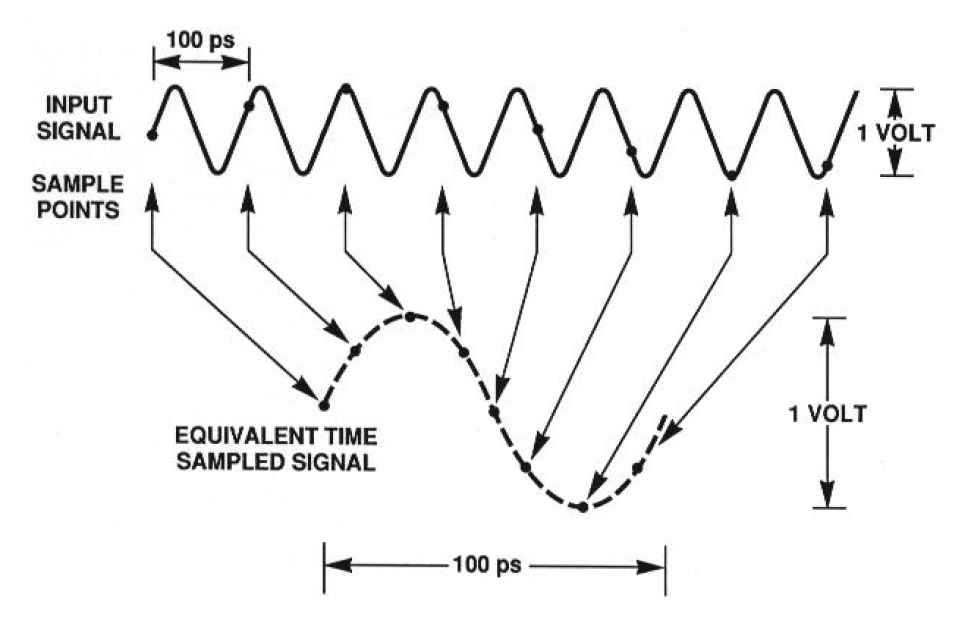
\includegraphics[width=0.9\textwidth]{SETS2.png}
\caption{Example equivalent time sampled signal.\cite{SETS}} 
\label{SETS2}
\end{figure}
\newpage

\subsection{Conclusion}
Different studies have shown that Received Signal Strength can theoretically measure distance accurately. However RSSI seems to be very unreliable in many circumstances which leads to not being viable for distance measurements with moving robots. 

Time Of Flight has been very promising, however using electromagnetic signals (For example RF, WI-FI or Bluetooth) the acceptable accuracy starts at from a minimum range of 1-2 meters which leads to unreliable to no useful information at all in the range of 1-2 meters. This minimum range could be narrowed using an Sequential Equivalent Time Sampling Circuit, however such a circuit is complex to develop. However using waveforms with a lower velocity propagation can lead to accurate close range measurements. In this case Time Of Flight suits better for the required use, being more accurate and reliable see figure \ref{RSSIvsTOF}.\cite{TOF}

\begin{figure}[H]
\centering
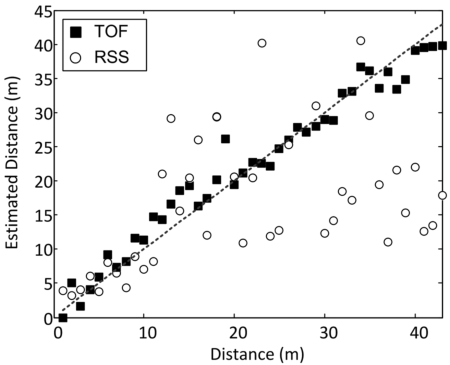
\includegraphics[width=0.9\textwidth]{RSSIvsTOF.pdf}
\caption{Accuracy RSSI vs TOF.\cite{TOF}} 
\label{RSSIvsTOF}
\end{figure}

Determining relative distance does not lead to localization to do so a angle is required to be continued... 
\newpage



\section{Propulsion,Actuators and Effectors}

In this chapter the sub-questions about the propulsion, actuators and effectors are researched and answered. First of all, the possible types of propulsion will be researched. Then the various kinds of actuators with a suitable effector will be considered. Depending on the situation different types of propulsion is used. For example a robot that operates in an environment with water would not be implemented with DC motor drivers and tyres. The robot build in this research should be able to operate on Mars in the future. Therefore the robot cant get stuck easily since that will cost millions, since the robot cannot complete his mission. Since swarming and not propulsion is the main goal of this research a simple way of locomotion would suffice. However there should be the possibility to implement a different kind of propulsion in the future, so that the robot can be used on Mars. 


%In dit hoofdstuk worden de deelvragen over de aandrijving, actuatoren en effectoren beantwoord. Allereerst zal er onderzocht worden welke soorten aandrijving er mogelijk zijn.Vervolgens zal er worden gekeken welke actuatoren er gebruikt kunnen worden en hoe de energie van de actuator gebruikt kan worden om de robot voort te bewegen. Als laatste wordt er gekeken welke effectoren nodig zijn. Robots worden op veel verschillende manier aangedreven, afhankelijk van de situatie.Bijvoorbeeld een robot die op het water moet opereren zal niet vaak met DC motoren met wielen worden ge\"implementeerd. In dit onderzoek kijken we naar een robot die in de toekomst mogelijk naar mars gestuurd kan worden. Dan kan de robot niet zomaar vast komen te zitten, aangezien er dan miljoenen voor niks verloren gaan. Omdat er eerst met een vereenvoudigde werkelijkheid wordt gewerkt is het vooral belangrijk dat de robot eenvoudig kan voortbewegen. Wel moet er ruimte zijn om later een andere module te kunnen aansluiten zodat hij ook op mars zich zou kunnen voortbewegen. 

\subsubsection{Effectors}
The way a robot moves is determined by its effector with his corresponding actuator. Possible types of effectors are:

%Door een effector aan een actuator de koppelen kan een robot zich voortbewegen. Mogelijke effectoren kunnen zijn:

\begin{itemize}
\item Wheels
\item Leg(s)
\item Catepillar tracks
\item Air cushion  
\item Propeller 
\item (Superconductor)
\end{itemize}

Each of these effectors have pro's and con's in different situations. Tyres are easily implemented, but there are various ways to implement these. The amount of tyres used will affect the handling of the robot. With a minimum two tyres, movement can already be realized. The downside is that driving with two wheels is not stable, only with algorithms that can balance the robot stable movement can be accomplished. It would be easier to implement more than two wheels so that the robot is more stable and movement is easier. 


  
%hier gebleven met vertalen
Elke van deze effectoren hebben voor en nadelen in verschillende situaties.\\Wielen zijn eenvoudig te implementeren, er kunnen verschillende aantallen wielen worden aangebracht. Het aantal wielen heeft wel invloed op het rijgedrag van de robot. Met twee wielen kan er worden gereden, mits de robot in balans wordt gehouden. Dit kan worden gedaan door middel van een zwenkwiel, of door een regelsysteem te bedenken dat de twee wielen de robot in balans houden. Dit laatste kost veel energie en is niet eenvoudig. Met drie wielen staat de robot al een stuk stabieler. Het nadeel hiervan is dat sturen soms moeizaam kan zijn. Met vier wielen is de robot nog stabieler en kan er op verschillende manieren worden gestuurd. De wielen kunnen tegengesteld worden aangedreven waardoor de robot draait. Dit kost wel meer energie dan nodig is aangezien er extra wrijving ontstaat. Een optie is de voorste wielen te laten draaien, waardoor de robot in de richting van de wielen zal voortbewegen. Zoals bij een auto het geval is. Dit is weer lastiger te implementeren aangezien er een soort van stuurmechanisme moet worden bedacht. 

\subsubsection{Actuatoren}

De keuze van de actuator hangt sterk samen met de effectoren.

\subsubsection{Aandrijving}

\newpage
\section{Swarm Communication}
There are several requirements to realise a robot swarm. Each member of the population needs to communicate with the rest of the swarm. To give the members full freedom of movement the communication also needs to be wireless. It is important that the population size of the swarm is dynamic, because of the scalability of the swarm. As mentioned earlier a swarm does not have a master. So each member needs to be capable to maintain the network. These networks also must be able to reroute around nodes that have been lost.

To create an network with those characteristics a (wireless) mesh network ((W)MN) is a possible solution. A mesh network relies on communication nodes in which data is distributed. All of the communication nodes cooperate in the distribution of data in the network. Each node of the network is connected to one or more nearby in range node(s) and forwards data on behalf of the other nodes. \cite{meshnetworking} A example of an mesh network is illustrated in figure \ref{fig:WMN}. To ensure a realiable network, self-organization and topology control alogorithms are needed.\cite{WMN1} Mesh networks can use self-healing algorithms such as Shortest Path Bridging (SPB) to restore and reroute the connection around broken nodes/clients. Shortest path bridging calculates the most favorable connections to the clients with the lowest path costs. \cite{SPB} Other usefull algorithms are listed in \cite{position-based}. The most efficient algorithm for path bridging depends on the situation where the clients are operating in which is described in \cite{position-based}.

A wireless mesh network (WMN) is a dynamically self-organized and configured network. \cite{WMN1} Each node or client in the network is able to create an ad hoc network to maintain the mesh connectivity, this is called client WMN's. These networks are able to reroute around nodes that have been lost. On large scale projects wireless mesh networks are costefficient because of the saving of wired connections.\cite{meshnetworking}

\begin{figure}[H]
   \centering
   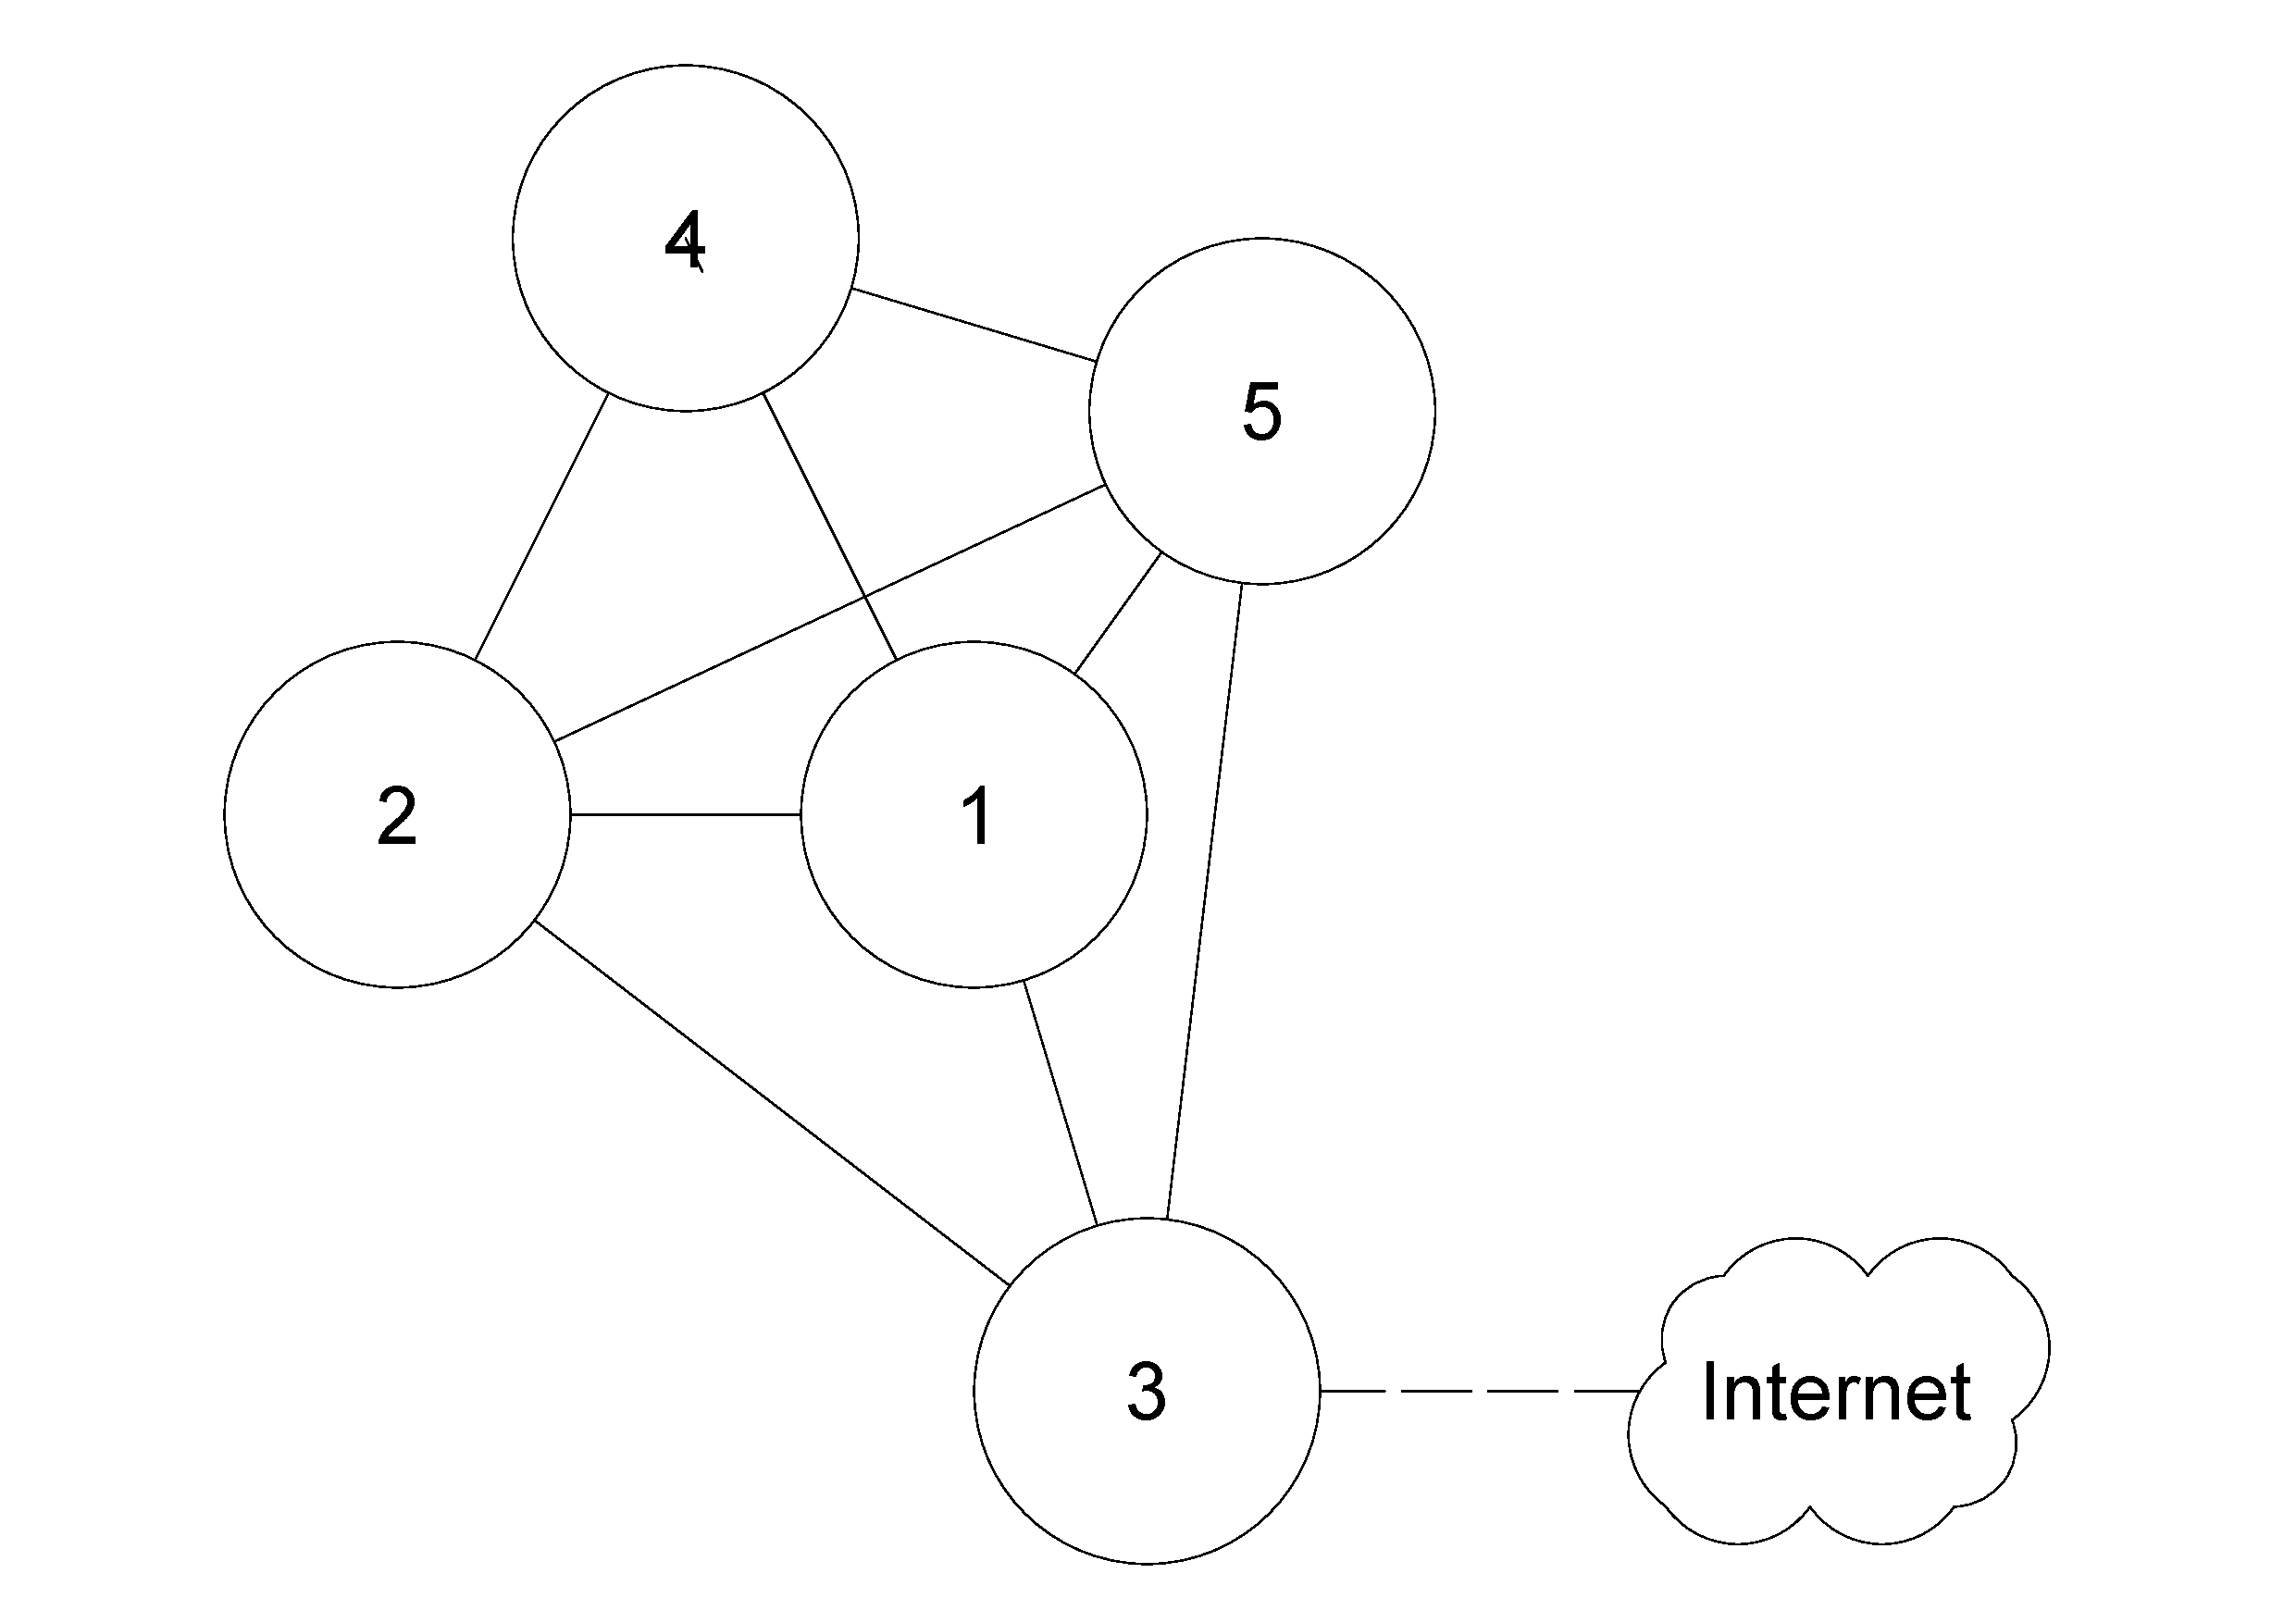
\includegraphics[width=1\textwidth]{WMN}
   \caption{An example of a wireless mesh network with 5 clients and an optional internet connection. The connections made in this example are random.}
   \label{fig:WMN}
\end{figure}




There exist several techniques to accomplish this method 
Examples of possible protocols:

% \begin{itemize}[noitemsep]
%     \item IEEE 802.11
%     \item ZigBee
%     \item SwarmBee
% \end{itemize}

\newpage


\subsection{Proximity sensor}

For close range obstacle avoidance (0m - 0,3m, the robots will need some kind of proximity sensing technique. The sensor needs to differentiate between different "treats" for the robot to function properly. For example; when the sensor detects a small hill, which the robot can move over it should not trigger the robot to move away from it. But when it detects a big obstacle it should trigger the robot to move away. This is important because the robots will eventually be expected to move across rough terrain (like Mars). In the next paragraphs some different proximity sensor techniques will be discussed. Price is also a important factor while comparing these techniques. Multiple robots must be made on a tight budget, so costs should be cut where possible.\\


\subsubsection{Ultrasonic sensor}
Ultrasonic sensors are widely used in robotics for proximity sensing. An ultrasonic sensor uses the time of flight (TOF) to operate. It sends out an ultrasonic sound wave and measures the time it takes for the sound to be reflected back. The speed of the sound is known so the distance can be calculated. The fact that this method uses sound is a big advantage when measuring small distances. Sound has a velocity of propagation of around 340 m/s. Most other methods use signals that travel with the speed of light ( $3\cdot10^{8}$). The problem with the high velocity of  propagation especially with measuring distances shorter than one meter is that the TOF will be in terms of a few nanoseconds.  The hardware needed to process signals with this kind of speed will require more complex circuit design and ultimately cost more. The ultrasonic signal that is received after reflected from an object hold information about the shape and size of the object. This can be used to discriminate between different obstacles\cite{ultraobject}. Because there's a diffrent atmosphere on Mars ultrasonic sound gets heavily dappened \cite{soundonmars}. This mean that this method wont be usable on Mars itself. A pro of the ultrasonic sensor is the low cost. A sensor with specified for short distances costs between 2\euro and 10\euro.


\subsubsection{Lidar sensor}
Light detection and ranging (lidar) works with the same principle as the ultrasonic sensor. It uses time of flight to determine the distance from an object. Instead of sound it uses the light of a laser as its medium. Lidar can be used for various applications like: 3D modeling of an environment, weather forecast and distance measurements \cite{whatlidar}. Lidar is a proven technology on Mars, it has been used on the Phoenix mission to measure clouds and atmospheric dust \cite{lidarmars}. A lidar suitable for the purpose of proximity sensing would be de Lidar lite v2. This is a proximity sensor designed for robotics. It has a range 0-40m and an accuracy of +/- 0,025m. Being the cheapest lidar sensor on the market it still costs 100\euro. Object discrimination with the Lidar lite is not possible due to the limited information. More complex lidar systems with a moving laser could be able to discriminate and detect objects really precise, but this requires really complex systems.


\begin{figure}[!ht]

  \centering
      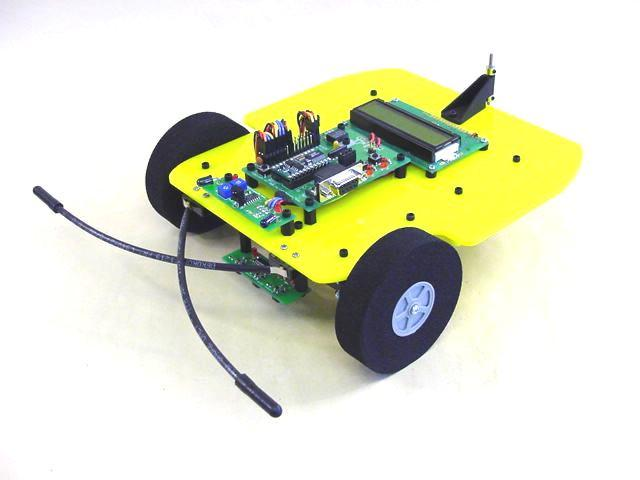
\includegraphics[width=0.5\textwidth]{voelsprieten.jpg}
  \caption{Robot met mechanische proximity sensor}  \label{voelspriet}
 
\end{figure}

\subsubsection{Mechanische sensor}
A mechanical sensor will consist of two important parts. The actuator, this could be a simple switch sensitive to a certain pressure. And the so called "arm" or "bumper", this is the part that makes contact with the obstacle's surface and works the mechanical force on the actuator. The beauty of this system is it's simplicity. There's no fast signals with different frequencies to be processed, just a simple on or of signal is all that needs to be observed. Due this limited input object discrimination wont be possible. Also robots bumping into object and each other is not a preferable situation. The robots might get stuck or break down.



\subsubsection{Sensor choice for the robot}
Now the question is which of the different sensor techniques proposed, is the best to implement on the swarm robots. While answering this question the following points will be taken into account:

\begin{itemize}
    \item The sensor must be easy to reproduce because multiple robots must be made from the swarm.
    \item The budget is limited, therefore the sensor price should be cheap compared the the total price of one robot.
    \item Energy usage should be as low as possible to increase the operation time per robot.
    \item For budget reasons there has been chosen to not take into account if the sensor would work on Mars.
    \item It must be possible to discriminate between different obstacles.
\end{itemize}

Looking at these points it becomes clear that the lidar sensor wouldn't be the best choice. It doesn't really have any outstanding pros compared to the other two techniques and it's much more expensive. . As talked about before the mechanical sensor has a few drawbacks compared to the ultrasonic sensor. For these reasons the ultrasonic sensor seems the best choice. The only issue left to solve is how to sense the difference between obstacles which the robot has to avoid, and things the robot doesn't have to avoid, but still might be detected by the sensor. This will be discussed in the next paragraph.

\subsubsection{Obstacle discrimination with an ultrasonic sensor}
An ultrasonic sensor is usually used to detect if there is some obstacle in the way. In this case there is made no difference made between a obstacle that the robot can move over, or a obstacle that should be avoided. For example: a small slope or hill might be detected as an obstacle, but in truth the robot can move over it. The robots developed for this program will eventually be able to cross harsh terrain. In this case the proximity sensor will need to discriminate between these situations. Working with ultrasonic waves there are multiple domains to work with. These are time, frequency and amplitude. Time is used to determine the distance between the object and the sensor. The change in frequency and/or amplitude contains information about the shape of the object\cite{ultraobject}see figure \ref{ultrafreq}. In the paper "Object recognition with ultrasonic sensor" is concluded that looking at the amplitude over time contains enough information to discriminate between object\cite{ultraobject}. The example is given of an object with separated surfaces of 3,5 cm, the echo from the second surface will be delayed by 0,2 msec relative to the echo from the first surface. This delay can be easily detected with a microprocessor. The reason looking at frequency isn't the first choice is because of the higher hardware requirements it would require to properly sample the ultrasonic signal. Looking at amplitude and time does not require the signal to be sampled at the Nyquist rate so lower clock rate microprocessors can be used to do the processing.
\\
\begin{figure}[h]

  \centering
      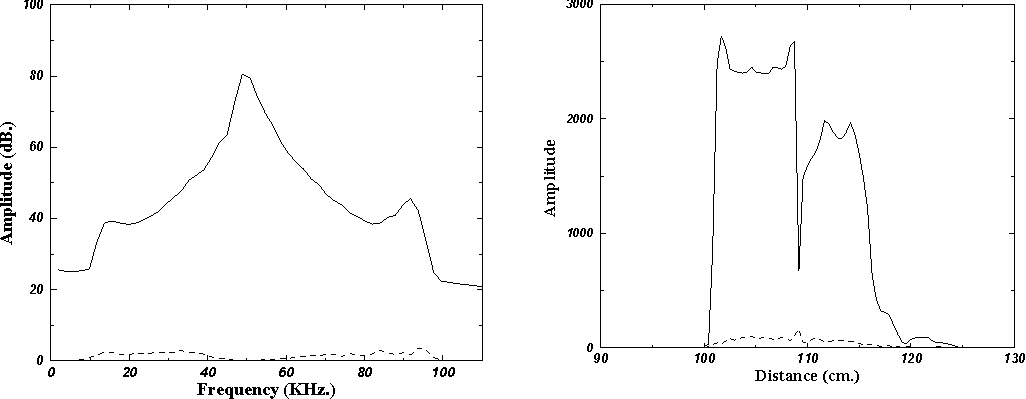
\includegraphics[width=1\textwidth]{ultrafreq.pdf}
  \caption{The left graph shows the average PSD from 50 echos generated by a plastic botthle from a distance of 100cm, the average envelope is generated using 50 echos of the same bottle} \cite{ultraobject}  \label{ultrafreq}
 
\end{figure}


\newpage

\section{Bibliografie}
\bibliography{references}
\bibliographystyle{IEEEtran}



\end{document}